% Options for packages loaded elsewhere
\PassOptionsToPackage{unicode}{hyperref}
\PassOptionsToPackage{hyphens}{url}
%
\documentclass[
]{book}
\usepackage{lmodern}
\usepackage{amssymb,amsmath}
\usepackage{ifxetex,ifluatex}
\ifnum 0\ifxetex 1\fi\ifluatex 1\fi=0 % if pdftex
  \usepackage[T1]{fontenc}
  \usepackage[utf8]{inputenc}
  \usepackage{textcomp} % provide euro and other symbols
\else % if luatex or xetex
  \usepackage{unicode-math}
  \defaultfontfeatures{Scale=MatchLowercase}
  \defaultfontfeatures[\rmfamily]{Ligatures=TeX,Scale=1}
\fi
% Use upquote if available, for straight quotes in verbatim environments
\IfFileExists{upquote.sty}{\usepackage{upquote}}{}
\IfFileExists{microtype.sty}{% use microtype if available
  \usepackage[]{microtype}
  \UseMicrotypeSet[protrusion]{basicmath} % disable protrusion for tt fonts
}{}
\makeatletter
\@ifundefined{KOMAClassName}{% if non-KOMA class
  \IfFileExists{parskip.sty}{%
    \usepackage{parskip}
  }{% else
    \setlength{\parindent}{0pt}
    \setlength{\parskip}{6pt plus 2pt minus 1pt}}
}{% if KOMA class
  \KOMAoptions{parskip=half}}
\makeatother
\usepackage{xcolor}
\IfFileExists{xurl.sty}{\usepackage{xurl}}{} % add URL line breaks if available
\IfFileExists{bookmark.sty}{\usepackage{bookmark}}{\usepackage{hyperref}}
\hypersetup{
  pdftitle={An analysis of Cryptocurrency},
  pdfauthor={Timothy McCormack, Carolyn Herrera, Wei Chun Tien,},
  hidelinks,
  pdfcreator={LaTeX via pandoc}}
\urlstyle{same} % disable monospaced font for URLs
\usepackage{color}
\usepackage{fancyvrb}
\newcommand{\VerbBar}{|}
\newcommand{\VERB}{\Verb[commandchars=\\\{\}]}
\DefineVerbatimEnvironment{Highlighting}{Verbatim}{commandchars=\\\{\}}
% Add ',fontsize=\small' for more characters per line
\usepackage{framed}
\definecolor{shadecolor}{RGB}{248,248,248}
\newenvironment{Shaded}{\begin{snugshade}}{\end{snugshade}}
\newcommand{\AlertTok}[1]{\textcolor[rgb]{0.94,0.16,0.16}{#1}}
\newcommand{\AnnotationTok}[1]{\textcolor[rgb]{0.56,0.35,0.01}{\textbf{\textit{#1}}}}
\newcommand{\AttributeTok}[1]{\textcolor[rgb]{0.77,0.63,0.00}{#1}}
\newcommand{\BaseNTok}[1]{\textcolor[rgb]{0.00,0.00,0.81}{#1}}
\newcommand{\BuiltInTok}[1]{#1}
\newcommand{\CharTok}[1]{\textcolor[rgb]{0.31,0.60,0.02}{#1}}
\newcommand{\CommentTok}[1]{\textcolor[rgb]{0.56,0.35,0.01}{\textit{#1}}}
\newcommand{\CommentVarTok}[1]{\textcolor[rgb]{0.56,0.35,0.01}{\textbf{\textit{#1}}}}
\newcommand{\ConstantTok}[1]{\textcolor[rgb]{0.00,0.00,0.00}{#1}}
\newcommand{\ControlFlowTok}[1]{\textcolor[rgb]{0.13,0.29,0.53}{\textbf{#1}}}
\newcommand{\DataTypeTok}[1]{\textcolor[rgb]{0.13,0.29,0.53}{#1}}
\newcommand{\DecValTok}[1]{\textcolor[rgb]{0.00,0.00,0.81}{#1}}
\newcommand{\DocumentationTok}[1]{\textcolor[rgb]{0.56,0.35,0.01}{\textbf{\textit{#1}}}}
\newcommand{\ErrorTok}[1]{\textcolor[rgb]{0.64,0.00,0.00}{\textbf{#1}}}
\newcommand{\ExtensionTok}[1]{#1}
\newcommand{\FloatTok}[1]{\textcolor[rgb]{0.00,0.00,0.81}{#1}}
\newcommand{\FunctionTok}[1]{\textcolor[rgb]{0.00,0.00,0.00}{#1}}
\newcommand{\ImportTok}[1]{#1}
\newcommand{\InformationTok}[1]{\textcolor[rgb]{0.56,0.35,0.01}{\textbf{\textit{#1}}}}
\newcommand{\KeywordTok}[1]{\textcolor[rgb]{0.13,0.29,0.53}{\textbf{#1}}}
\newcommand{\NormalTok}[1]{#1}
\newcommand{\OperatorTok}[1]{\textcolor[rgb]{0.81,0.36,0.00}{\textbf{#1}}}
\newcommand{\OtherTok}[1]{\textcolor[rgb]{0.56,0.35,0.01}{#1}}
\newcommand{\PreprocessorTok}[1]{\textcolor[rgb]{0.56,0.35,0.01}{\textit{#1}}}
\newcommand{\RegionMarkerTok}[1]{#1}
\newcommand{\SpecialCharTok}[1]{\textcolor[rgb]{0.00,0.00,0.00}{#1}}
\newcommand{\SpecialStringTok}[1]{\textcolor[rgb]{0.31,0.60,0.02}{#1}}
\newcommand{\StringTok}[1]{\textcolor[rgb]{0.31,0.60,0.02}{#1}}
\newcommand{\VariableTok}[1]{\textcolor[rgb]{0.00,0.00,0.00}{#1}}
\newcommand{\VerbatimStringTok}[1]{\textcolor[rgb]{0.31,0.60,0.02}{#1}}
\newcommand{\WarningTok}[1]{\textcolor[rgb]{0.56,0.35,0.01}{\textbf{\textit{#1}}}}
\usepackage{longtable,booktabs}
% Correct order of tables after \paragraph or \subparagraph
\usepackage{etoolbox}
\makeatletter
\patchcmd\longtable{\par}{\if@noskipsec\mbox{}\fi\par}{}{}
\makeatother
% Allow footnotes in longtable head/foot
\IfFileExists{footnotehyper.sty}{\usepackage{footnotehyper}}{\usepackage{footnote}}
\makesavenoteenv{longtable}
\usepackage{graphicx,grffile}
\makeatletter
\def\maxwidth{\ifdim\Gin@nat@width>\linewidth\linewidth\else\Gin@nat@width\fi}
\def\maxheight{\ifdim\Gin@nat@height>\textheight\textheight\else\Gin@nat@height\fi}
\makeatother
% Scale images if necessary, so that they will not overflow the page
% margins by default, and it is still possible to overwrite the defaults
% using explicit options in \includegraphics[width, height, ...]{}
\setkeys{Gin}{width=\maxwidth,height=\maxheight,keepaspectratio}
% Set default figure placement to htbp
\makeatletter
\def\fps@figure{htbp}
\makeatother
\setlength{\emergencystretch}{3em} % prevent overfull lines
\providecommand{\tightlist}{%
  \setlength{\itemsep}{0pt}\setlength{\parskip}{0pt}}
\setcounter{secnumdepth}{5}
\usepackage{booktabs}
\usepackage{amsthm}
\makeatletter
\def\thm@space@setup{%
  \thm@preskip=8pt plus 2pt minus 4pt
  \thm@postskip=\thm@preskip
}
\makeatother
\usepackage{booktabs}
\usepackage{longtable}
\usepackage{array}
\usepackage{multirow}
\usepackage{wrapfig}
\usepackage{float}
\usepackage{colortbl}
\usepackage{pdflscape}
\usepackage{tabu}
\usepackage{threeparttable}
\usepackage{threeparttablex}
\usepackage[normalem]{ulem}
\usepackage{makecell}
\usepackage[]{natbib}
\bibliographystyle{apalike}

\title{An analysis of Cryptocurrency}
\author{Timothy McCormack, Carolyn Herrera, Wei Chun Tien,}
\date{2020-11-09}

\begin{document}
\maketitle

{
\setcounter{tocdepth}{1}
\tableofcontents
}
\hypertarget{preface}{%
\chapter*{Preface}\label{preface}}
\addcontentsline{toc}{chapter}{Preface}

\hypertarget{intro}{%
\chapter{Introduction}\label{intro}}

\hypertarget{data-import-and-clean}{%
\chapter{Data Import and Clean}\label{data-import-and-clean}}

\begin{Shaded}
\begin{Highlighting}[]
\KeywordTok{library}\NormalTok{(tidyverse)}
\KeywordTok{library}\NormalTok{(tidytext)}
\KeywordTok{library}\NormalTok{(textclean)}
\KeywordTok{library}\NormalTok{(dplyr)}
\KeywordTok{library}\NormalTok{(stringr)}
\KeywordTok{library}\NormalTok{(knitr)}
\KeywordTok{library}\NormalTok{(wordcloud)}
\KeywordTok{library}\NormalTok{(kableExtra)}
\KeywordTok{library}\NormalTok{(DT)}
\KeywordTok{library}\NormalTok{(tidygraph)}
\KeywordTok{library}\NormalTok{(ggraph)}
\KeywordTok{library}\NormalTok{(tm)}
\end{Highlighting}
\end{Shaded}

\begin{Shaded}
\begin{Highlighting}[]
\NormalTok{knitr}\OperatorTok{::}\NormalTok{opts_chunk}\OperatorTok{$}\KeywordTok{set}\NormalTok{(}\DataTypeTok{message =} \OtherTok{FALSE}\NormalTok{, }\DataTypeTok{warning =} \OtherTok{FALSE}\NormalTok{, }\DataTypeTok{echo =} \OtherTok{TRUE}\NormalTok{)}
\CommentTok{# set to TRUE to run this on only one reference file}
\NormalTok{debugging <-}\StringTok{ }\OtherTok{FALSE}
\CommentTok{# this will expect the file or files to be in a subdirectory with the following name}
\NormalTok{refsource <-}\StringTok{ "MungingProj2"}
\NormalTok{dataDir <-}\StringTok{ "Proj2Data"}
\NormalTok{workingDir <-}\StringTok{ }\NormalTok{refsource}

\CommentTok{# prefixes for all File reads and writes}
\CommentTok{# titles for tables}
\NormalTok{titletext <-}\StringTok{ "RedditCrypto"}
\NormalTok{srs =}\StringTok{ }\KeywordTok{c}\NormalTok{(}\StringTok{"CryptoCurrency"}\NormalTok{,}\StringTok{"CryptoMarkets"}\NormalTok{)}

\StringTok{`}\DataTypeTok\StringTok{`}\NormalTok{ <-}\StringTok{ }\KeywordTok{Negate}\NormalTok{(}\StringTok{`}\DataTypeTok\StringTok{`}\NormalTok{)}
\end{Highlighting}
\end{Shaded}

\hypertarget{import-data}{%
\section{Import Data}\label{import-data}}

\begin{Shaded}
\begin{Highlighting}[]
\NormalTok{subm_fnames <-}\StringTok{ }\KeywordTok{list.files}\NormalTok{(dataDir, }\DataTypeTok{pattern =} \StringTok{"*_submissions.csv"}\NormalTok{, }\DataTypeTok{full.names =} \OtherTok{TRUE}\NormalTok{)}
\NormalTok{comm_fnames <-}\StringTok{ }\KeywordTok{list.files}\NormalTok{(dataDir, }\DataTypeTok{pattern =} \StringTok{"*_comments.csv"}\NormalTok{, }\DataTypeTok{full.names =} \OtherTok{TRUE}\NormalTok{)}
\NormalTok{subr_fnames <-}\StringTok{ }\KeywordTok{list.files}\NormalTok{(dataDir, }\DataTypeTok{pattern =} \StringTok{"*_subreddit.csv"}\NormalTok{, }\DataTypeTok{full.names =} \OtherTok{TRUE}\NormalTok{)}

\ControlFlowTok{for}\NormalTok{ (i }\ControlFlowTok{in} \DecValTok{1}\OperatorTok{:}\KeywordTok{length}\NormalTok{(subm_fnames)) }
  \KeywordTok{assign}\NormalTok{(srs[i], }\KeywordTok{read.csv}\NormalTok{(subm_fnames[i]))}
\NormalTok{SubmData<-}\StringTok{ }\KeywordTok{rbind}\NormalTok{(CryptoCurrency, CryptoMarkets)}
\ControlFlowTok{for}\NormalTok{ (i }\ControlFlowTok{in} \DecValTok{1}\OperatorTok{:}\KeywordTok{length}\NormalTok{(comm_fnames)) }
  \KeywordTok{assign}\NormalTok{(srs[i], }\KeywordTok{read.csv}\NormalTok{(comm_fnames[i]))}
\NormalTok{CommData<-}\StringTok{ }\KeywordTok{rbind}\NormalTok{(CryptoCurrency, CryptoMarkets)}
\ControlFlowTok{for}\NormalTok{ (i }\ControlFlowTok{in} \DecValTok{1}\OperatorTok{:}\KeywordTok{length}\NormalTok{(subr_fnames)) }
  \KeywordTok{assign}\NormalTok{(srs[i], }\KeywordTok{read.csv}\NormalTok{(subr_fnames[i]))}
\NormalTok{SubrData<-}\StringTok{ }\KeywordTok{rbind}\NormalTok{(CryptoCurrency, CryptoMarkets)}
\end{Highlighting}
\end{Shaded}

\hypertarget{fix-names}{%
\subsection{Fix Names}\label{fix-names}}

\begin{Shaded}
\begin{Highlighting}[]
\NormalTok{srs <-}\StringTok{ }\KeywordTok{unique}\NormalTok{(SubmData}\OperatorTok{$}\NormalTok{subreddit)}

\NormalTok{SubmData <-}\StringTok{ }\NormalTok{SubmData }\OperatorTok
\StringTok{    }\KeywordTok{mutate}\NormalTok{(}
      \DataTypeTok{subreddit =} \KeywordTok{case_when}\NormalTok{(}
\NormalTok{        .}\OperatorTok{$}\NormalTok{subreddit }\OperatorTok{==}\StringTok{ }\NormalTok{srs[}\DecValTok{1}\NormalTok{] }\OperatorTok{~}\StringTok{ "r/CryptoCurrency"}\NormalTok{,}
\NormalTok{        .}\OperatorTok{$}\NormalTok{subreddit }\OperatorTok{==}\StringTok{ }\NormalTok{srs[}\DecValTok{2}\NormalTok{] }\OperatorTok{~}\StringTok{ "r/CryptoMarkets"}\NormalTok{)}
\NormalTok{      ) }\OperatorTok
\StringTok{  }\KeywordTok{ungroup}\NormalTok{()}
\end{Highlighting}
\end{Shaded}

\hypertarget{data-collection}{%
\section{Data Collection}\label{data-collection}}

\begin{Shaded}
\begin{Highlighting}[]
\NormalTok{submnums <-}\StringTok{ }\KeywordTok{table}\NormalTok{(SubmData}\OperatorTok{$}\NormalTok{subreddit)}
\NormalTok{SubmNums <-}\StringTok{ }\KeywordTok{as.data.frame}\NormalTok{(submnums, }\DataTypeTok{.name_repair =} \StringTok{"minimal"}\NormalTok{)}
\KeywordTok{colnames}\NormalTok{(SubmNums)[}\DecValTok{1}\NormalTok{] <-}\StringTok{ "Subreddit"}
\KeywordTok{ggplot}\NormalTok{(SubmNums, }\KeywordTok{aes}\NormalTok{(}\DataTypeTok{x =}\NormalTok{ Subreddit, }\DataTypeTok{y =}\NormalTok{ Freq, }\DataTypeTok{fill =}\NormalTok{ Subreddit)) }\OperatorTok{+}\StringTok{ }\KeywordTok{geom_bar}\NormalTok{(}\DataTypeTok{stat =} \StringTok{"identity"}\NormalTok{) }\OperatorTok{+}\StringTok{ }\KeywordTok{scale_y_continuous}\NormalTok{(}\DataTypeTok{name=}\StringTok{"# of Submissions by Subreddit"}\NormalTok{, }\DataTypeTok{labels =}\NormalTok{ scales}\OperatorTok{::}\NormalTok{comma)}
\end{Highlighting}
\end{Shaded}

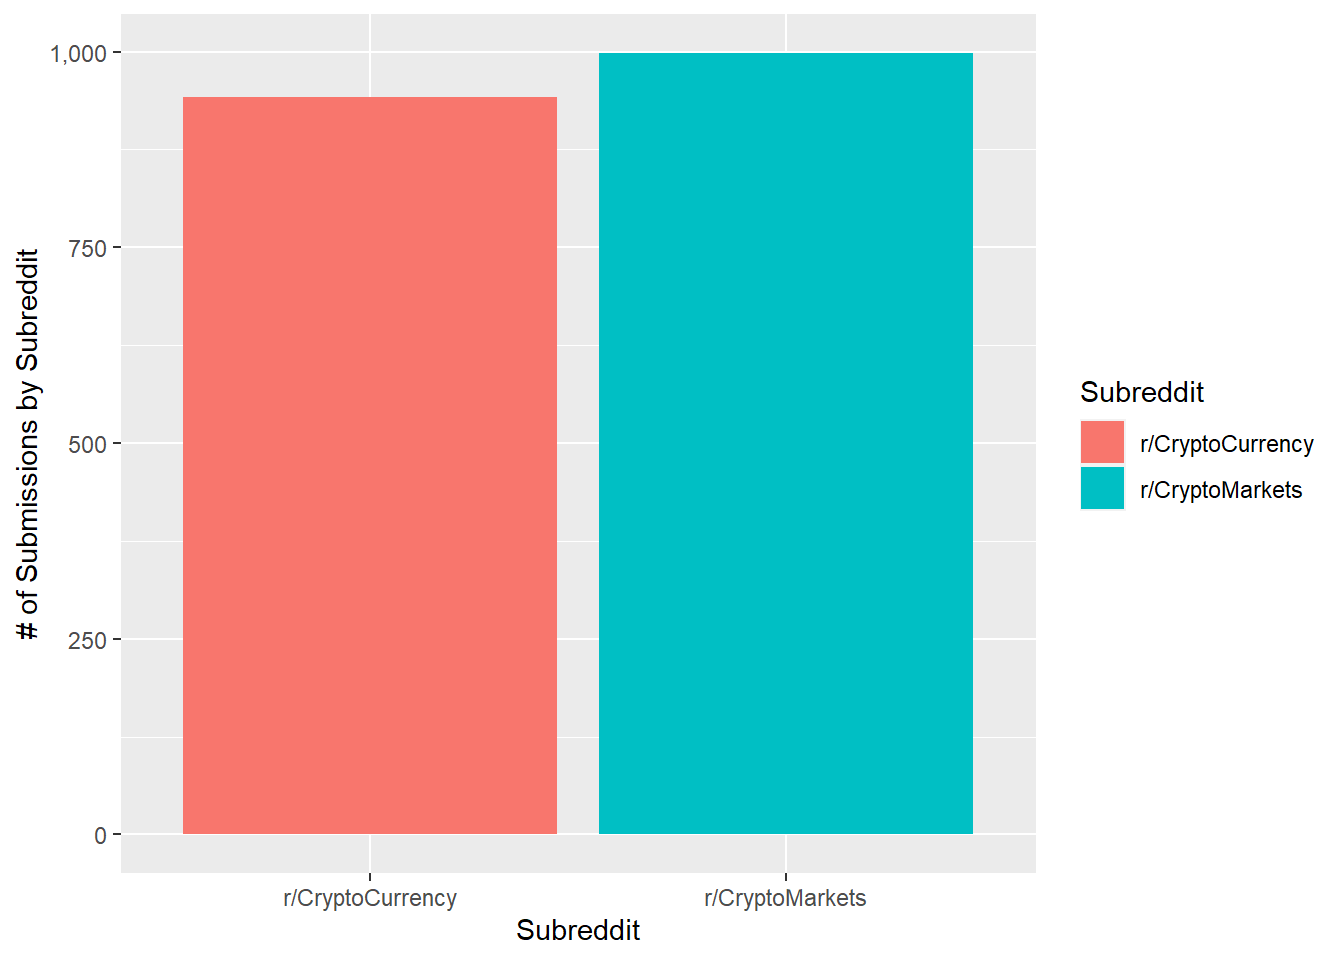
\includegraphics{bookdown-demo_files/figure-latex/unnamed-chunk-5-1.pdf}

\begin{Shaded}
\begin{Highlighting}[]
\NormalTok{c <-}\StringTok{ }\NormalTok{CommData}

\NormalTok{commnums <-}\StringTok{ }\KeywordTok{table}\NormalTok{(c}\OperatorTok{$}\NormalTok{subreddit)}
\NormalTok{CommNums <-}\StringTok{ }\KeywordTok{as.data.frame}\NormalTok{(commnums, }\DataTypeTok{.name_repair =} \StringTok{"minimal"}\NormalTok{)}
\KeywordTok{colnames}\NormalTok{(CommNums)[}\DecValTok{1}\NormalTok{] <-}\StringTok{ "Subreddit"}
\KeywordTok{ggplot}\NormalTok{(CommNums, }\KeywordTok{aes}\NormalTok{(}\DataTypeTok{x =}\NormalTok{ Subreddit, }\DataTypeTok{y =}\NormalTok{ Freq, }\DataTypeTok{fill =}\NormalTok{ Subreddit)) }\OperatorTok{+}\StringTok{ }\KeywordTok{geom_bar}\NormalTok{(}\DataTypeTok{stat =} \StringTok{"identity"}\NormalTok{) }\OperatorTok{+}\StringTok{ }\KeywordTok{scale_y_continuous}\NormalTok{(}\DataTypeTok{name=}\StringTok{"# of Comments by Subreddit (from 300 posts each)"}\NormalTok{, }\DataTypeTok{labels =}\NormalTok{ scales}\OperatorTok{::}\NormalTok{comma)}
\end{Highlighting}
\end{Shaded}

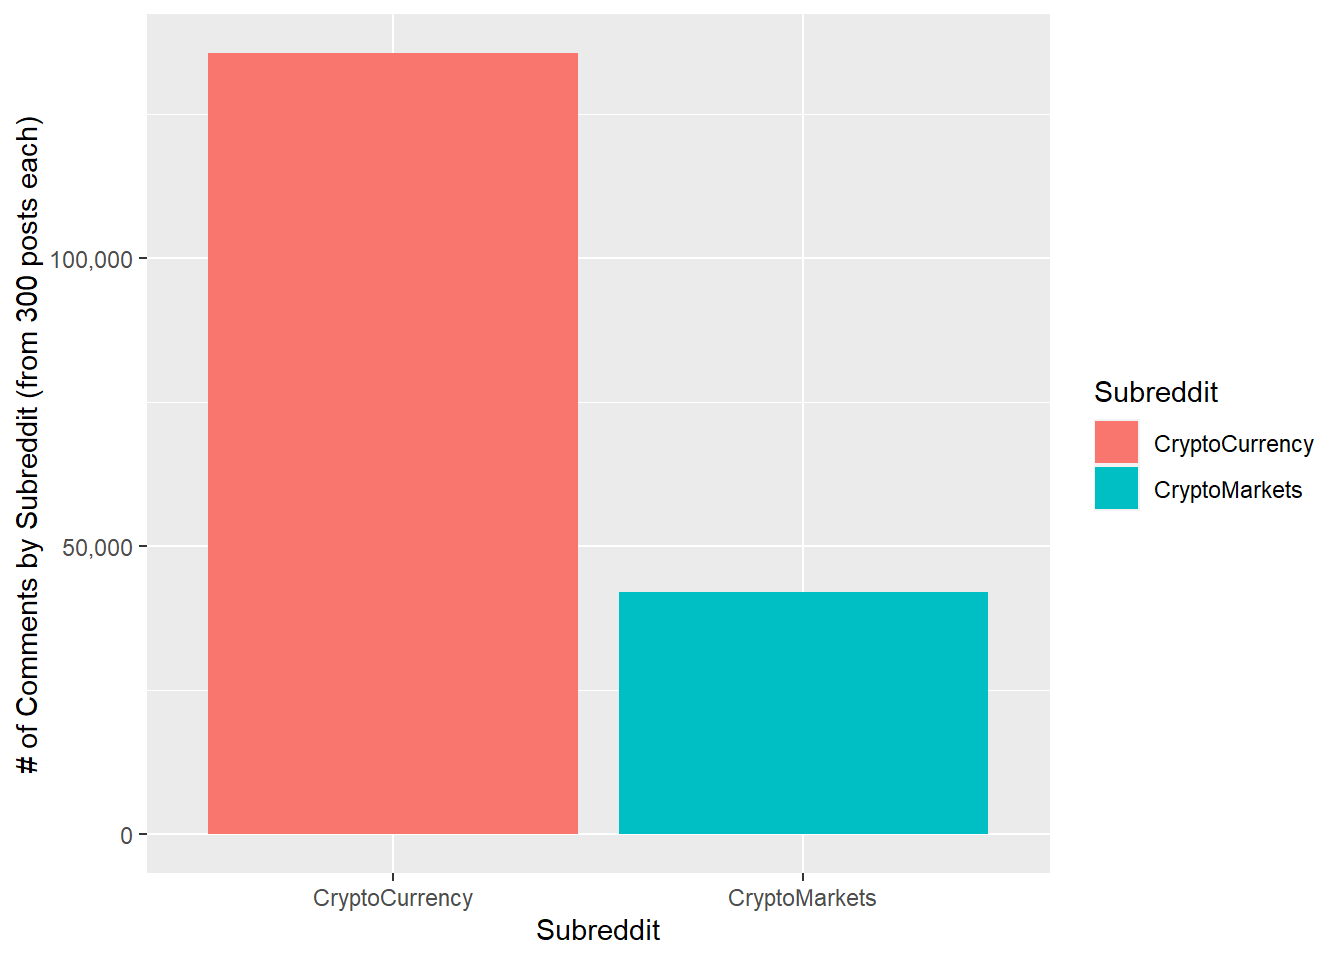
\includegraphics{bookdown-demo_files/figure-latex/unnamed-chunk-6-1.pdf}

\begin{Shaded}
\begin{Highlighting}[]
\KeywordTok{kable}\NormalTok{(SubrData) }\OperatorTok
\StringTok{  }\KeywordTok{kable_styling}\NormalTok{(}\StringTok{"striped"}\NormalTok{, }\DataTypeTok{full_width =}\NormalTok{ F)}
\end{Highlighting}
\end{Shaded}

\begin{table}[H]
\centering
\begin{tabular}{r|l|r|l|l}
\hline
X & title & subscribers & created & public\_description\\
\hline
0 & Cryptocurrency News \& Discussion & 1117855 & 2013-03-11 17:51:50 & The official source for CryptoCurrency News, Discussion \& Analysis.\\
\hline
0 & r/CryptoMarkets & 236835 & 2013-11-12 18:50:17 & FOREX community for cryptocurrencies. 

Tags: mt gox bitcoin, long term potential, open source exchange, low inflation rate, demand and price, technical analysis, fundamentals, Bitcoin, Ethereum, Litecoin, Monero, Dash, Augur, token, volume, oscillator, RSI, stochastic, trend, sentiment, strategy, scam, coin, coinmarketcap, altcoin, Peercoin, script, blockchain, PoW, PoS, Proof of Work,\\
\hline
\end{tabular}
\end{table}

\emph{Submissions} from each subreddit:

\emph{Comments} in each subreddit:

\hypertarget{clean}{%
\section{Clean}\label{clean}}

To ensure that our data accurately represent activity within the communitas, we want to ensure that each observation is a unique instance of engagement. Reposts tend to be common on reddit, so using a \texttt{distinct()} function on the text column will remove any duplicate posts. Additionally, any posts that are removed from the subreddits return an \texttt{NA} value in \texttt{user} column, thus we can remove deleted comments by filtering out all non \texttt{user\ ==\ NA}.

\begin{Shaded}
\begin{Highlighting}[]
\CommentTok{#Clean}
\KeywordTok{Encoding}\NormalTok{(SubmData}\OperatorTok{$}\NormalTok{text) <-}\StringTok{ "UTF-8"}

\NormalTok{Submissions <-}\StringTok{ }\NormalTok{SubmData }\OperatorTok
\StringTok{  }\KeywordTok{group_by}\NormalTok{(user) }\OperatorTok
\StringTok{    }\KeywordTok{filter}\NormalTok{(}\OperatorTok{!}\KeywordTok{is.na}\NormalTok{(user)) }\OperatorTok\StringTok{ }\CommentTok{# Take out deleted comments}
\StringTok{    }\KeywordTok{ungroup}\NormalTok{() }\OperatorTok
\StringTok{    }\KeywordTok{distinct}\NormalTok{(text, }\DataTypeTok{.keep_all =} \OtherTok{TRUE}\NormalTok{) }\CommentTok{#remove duplicate submissions}

\KeywordTok{paste}\NormalTok{(}\StringTok{"Removed"}\NormalTok{, }\KeywordTok{nrow}\NormalTok{(SubmData) }\OperatorTok{-}\StringTok{ }\KeywordTok{nrow}\NormalTok{(Submissions),}\StringTok{"submissions."}\NormalTok{)}
\end{Highlighting}
\end{Shaded}

\begin{verbatim}
## [1] "Removed 14 submissions."
\end{verbatim}

\hypertarget{submissions}{%
\subsection{Submissions}\label{submissions}}

The analysis of langauge begins by quantifying the presence of words in each Subm, through the process of \emph{tokenization}. \emph{Tokens} are discrete strings of words or characters that can be isolated as n-grams; with \emph{n} pertaining to the number of words in each token. Tokens are pulled from the body of text that is most informative for the purposes of analysis. For submissions, the informative text is the \emph{title} of the submission, which contains information on topics; whereas, for comments, the informative text is the \texttt{comment} itself.

\begin{Shaded}
\begin{Highlighting}[]
\KeywordTok{data}\NormalTok{(stop_words)}

\NormalTok{SubmissionTkns <-}\StringTok{ }\NormalTok{Submissions }\OperatorTok
\StringTok{  }\KeywordTok{group_by}\NormalTok{(subreddit) }\OperatorTok
\StringTok{    }\KeywordTok{unnest_tokens}\NormalTok{(word, text) }\OperatorTok
\StringTok{    }\KeywordTok{ungroup}\NormalTok{()}

\CommentTok{#G2Subm <- Submissions %>%}
\CommentTok{#    group_by(subreddit) %>%}
\CommentTok{#    unnest_tokens(bigram, text, token = "ngrams", n = 2, n_min = #2) %>% #repeat above as bigram}
\CommentTok{#    ungroup()}
\end{Highlighting}
\end{Shaded}

As part of the tokenization process for submissions, we remove stop words (e.g.~``and'', ``a'', ``the'') because we are interested in using our tokens to identify prevalent topics of discussion and attitudes in the religiously affiliated social clusters. In contrast, stop words are not removed from text data in comments because they are useful in the analysis of linguistic sentiment and behavior.
\#\#\#\# 1-grams (Clean)

\begin{Shaded}
\begin{Highlighting}[]
\CommentTok{#Create object for numbers, so that we can remove them from the data}
\NormalTok{nums <-}\StringTok{ }\NormalTok{SubmissionTkns }\OperatorTok\StringTok{ }\KeywordTok{filter}\NormalTok{(}\KeywordTok{str_detect}\NormalTok{(word, }\StringTok{"^[0-9]"}\NormalTok{)) }\OperatorTok\StringTok{ }\KeywordTok{select}\NormalTok{(word) }\OperatorTok\StringTok{ }\KeywordTok{unique}\NormalTok{() }\CommentTok{#Source: https://richpauloo.github.io/2017-12-29-Using-tidytext-to-make-word-clouds/}

\NormalTok{SubmissionTkns <-}\StringTok{ }\NormalTok{SubmissionTkns }\OperatorTok
\StringTok{    }\KeywordTok{anti_join}\NormalTok{(stop_words, }\DataTypeTok{by =} \StringTok{"word"}\NormalTok{) }\OperatorTok
\StringTok{    }\KeywordTok{anti_join}\NormalTok{(nums, }\DataTypeTok{by =} \StringTok{"word"}\NormalTok{) }\OperatorTok
\StringTok{    }\KeywordTok{filter}\NormalTok{(}\OperatorTok{!}\KeywordTok{grepl}\NormalTok{(}\StringTok{"_"}\NormalTok{, .}\OperatorTok{$}\NormalTok{word))}

\NormalTok{G1Subm <-}\StringTok{ }\NormalTok{SubmissionTkns}
\end{Highlighting}
\end{Shaded}

\hypertarget{grams-clean}{%
\subsubsection{2-grams (Clean)}\label{grams-clean}}

2-gram code is not used in analysis due to unsolved cleaning error.

\begin{Shaded}
\begin{Highlighting}[]
\CommentTok{#G2Subm_separated <- G2Subm %>% #Separate bigrams to remove stopwords and transitional phrases}
\CommentTok{#  separate(bigram, c("word1", "word2"), sep = " ") #run boolean functions for cleaning on `word1` and `word2`}

\CommentTok{#G2Subm_filtered <- G2Subm_separated %>% }
\CommentTok{#  filter(!word1 %in% stop_words$word) %>% #remove stop words}
\CommentTok{#  filter(!word2 %in% stop_words$word) %>%}
\CommentTok{#  filter(!word1 == "NA") %>% #remove anomylous strings}
\CommentTok{#  filter(!word2 == "NA") %>%}
\CommentTok{#  filter(!word1 %in% nums) %>% #remove numbers}
\CommentTok{#  filter(!word2 %in% nums)}

\CommentTok{#G2Subm <- G2Subm_filtered %>% }
\CommentTok{#  unite(bigram, word1, word2, sep = " ")#reunify cleaned word columns}

\CommentTok{#G2Subm <- G2Subm[!grepl("_", G2Subm$bigram),]}

\CommentTok{#rm(G2Subm_separated)}
\CommentTok{#rm(G2Subm_filtered)}
\end{Highlighting}
\end{Shaded}

\hypertarget{count}{%
\subsection{Count}\label{count}}

Following tokenization, the presence of each n-gram is tallied within each communitas. The tallies are then sorted to show what the most frequently occuring words are in each category.

\begin{Shaded}
\begin{Highlighting}[]
\NormalTok{G1SubmCount <-}\StringTok{ }\NormalTok{G1Subm }\OperatorTok
\StringTok{    }\KeywordTok{group_by}\NormalTok{(subreddit) }\OperatorTok\StringTok{ }\CommentTok{#group words by affiliation label}
\StringTok{    }\KeywordTok{count}\NormalTok{(word, }\DataTypeTok{sort =} \OtherTok{FALSE}\NormalTok{) }\OperatorTok\StringTok{ }\CommentTok{#count and create column 'n'}
\StringTok{    }\KeywordTok{ungroup}\NormalTok{()}

\CommentTok{#G2SubmCount <- G2Subm %>% #repeat for bigrams}
\CommentTok{#    group_by(subreddit) %>%}
\CommentTok{#    count(bigram, sort = FALSE) %>%}
\CommentTok{#    ungroup() }

\KeywordTok{rm}\NormalTok{(G1Subm)}
\CommentTok{#rm(G2Subm)}
\end{Highlighting}
\end{Shaded}

\hypertarget{comments}{%
\section{Comments}\label{comments}}

The cleaning and tokenization process for comments is similar to that of submissions; however, a few extra steps must be taken considering the casual and conversational nature of reddit comments.

\textbf{NEED TO DO:} Additionally, the number of comments on each submission varies, so it will be important to standardize word counts across subreddits..

\hypertarget{clean-1}{%
\subsection{Clean}\label{clean-1}}

\begin{Shaded}
\begin{Highlighting}[]
\KeywordTok{Encoding}\NormalTok{(CommData}\OperatorTok{$}\NormalTok{text) <-}\StringTok{ "UTF-8"}

\NormalTok{Comments <-}\StringTok{ }\NormalTok{CommData }\OperatorTok
\StringTok{  }\KeywordTok{group_by}\NormalTok{(user) }\OperatorTok
\StringTok{    }\KeywordTok{filter}\NormalTok{(}\OperatorTok{!}\KeywordTok{is.na}\NormalTok{(user)) }\OperatorTok\StringTok{ }\CommentTok{# Take out deleted comments}
\StringTok{    }\KeywordTok{ungroup}\NormalTok{() }\OperatorTok
\StringTok{    }\KeywordTok{distinct}\NormalTok{(text, }\DataTypeTok{.keep_all =} \OtherTok{TRUE}\NormalTok{) }\CommentTok{#remove duplicate comments}

\KeywordTok{paste}\NormalTok{(}\StringTok{"Removed"}\NormalTok{, }\KeywordTok{nrow}\NormalTok{(CommData) }\OperatorTok{-}\StringTok{ }\KeywordTok{nrow}\NormalTok{(Comments),}\StringTok{"comments"}\NormalTok{)}
\end{Highlighting}
\end{Shaded}

\begin{verbatim}
## [1] "Removed 12771 comments"
\end{verbatim}

\begin{Shaded}
\begin{Highlighting}[]
\NormalTok{url_regex <-}\StringTok{ "http[s]?://(?:[a-zA-Z]|[0-9]|[$-_@.&+]|[!*}\CharTok{\textbackslash{}\textbackslash{}}\StringTok{(}\CharTok{\textbackslash{}\textbackslash{}}\StringTok{),]|(?:%[0-9a-fA-F][0-9a-fA-F]))+"}

\NormalTok{Comments}\OperatorTok{$}\NormalTok{text <-stringi}\OperatorTok{::}\KeywordTok{stri_trans_general}\NormalTok{(Comments}\OperatorTok{$}\NormalTok{text, }\StringTok{"latin-ascii"}\NormalTok{) }\CommentTok{#converts text encoding, otherwise the tokenizer won't retain contractions}

\NormalTok{Comments}\OperatorTok{$}\NormalTok{text <-}\StringTok{ }\KeywordTok{str_remove_all}\NormalTok{(Comments}\OperatorTok{$}\NormalTok{text, url_regex)}
\end{Highlighting}
\end{Shaded}

\hypertarget{tokenize}{%
\subsection{Tokenize}\label{tokenize}}

\begin{Shaded}
\begin{Highlighting}[]
\CommentTok{#tokenize}
\NormalTok{G1Comm <-}\StringTok{ }\NormalTok{Comments }\OperatorTok
\StringTok{  }\KeywordTok{unnest_tokens}\NormalTok{(word, text) }\CommentTok{# %>%}
    \CommentTok{#ungroup()}

\CommentTok{#G2Comm <- Comments %>%}
\CommentTok{#    #group_by(subreddit) %>%}
\CommentTok{#    unnest_tokens(bigram, text, token = #"ngrams", n = 2, n_min = 2) #%>% #repeat above as bigram}
    \CommentTok{#ungroup()}
\end{Highlighting}
\end{Shaded}

\hypertarget{grams}{%
\subsubsection{1-grams}\label{grams}}

\begin{Shaded}
\begin{Highlighting}[]
\CommentTok{#Create object for numbers, so that we can remove them from the data}
\NormalTok{nums <-}\StringTok{ }\NormalTok{G1Comm }\OperatorTok\StringTok{ }\KeywordTok{filter}\NormalTok{(}\KeywordTok{str_detect}\NormalTok{(word, }\StringTok{"^[0-9]"}\NormalTok{)) }\OperatorTok\StringTok{ }\KeywordTok{select}\NormalTok{(word) }\OperatorTok\StringTok{ }\KeywordTok{unique}\NormalTok{() }\CommentTok{#Source: https://richpauloo.github.io/2017-12-29-Using-tidytext-to-make-word-clouds/}

\NormalTok{Bots <-}\StringTok{ }\KeywordTok{filter}\NormalTok{(G1Comm, word }\OperatorTok{==}\StringTok{ "bot"}\NormalTok{)}

\KeywordTok{data}\NormalTok{(stop_words)}

\NormalTok{CommTkns <-}\StringTok{ }\NormalTok{G1Comm }\OperatorTok
\StringTok{    }\KeywordTok{anti_join}\NormalTok{(stop_words) }\OperatorTok\StringTok{ }\CommentTok{#take out stop words (i.e. 'a', 'an', 'of', 'the')}
\StringTok{    }\KeywordTok{anti_join}\NormalTok{(nums, }\DataTypeTok{by =} \StringTok{"word"}\NormalTok{) }\OperatorTok
\StringTok{    }\KeywordTok{filter}\NormalTok{(user }\OperatorTok\StringTok{ }\NormalTok{Bots}\OperatorTok{$}\NormalTok{user) }\OperatorTok
\StringTok{    }\KeywordTok{filter}\NormalTok{(}\OperatorTok{!}\KeywordTok{grepl}\NormalTok{(}\StringTok{"_"}\NormalTok{, .}\OperatorTok{$}\NormalTok{word))}
    \CommentTok{#ungroup()}

\NormalTok{G1Comm <-}\StringTok{ }\NormalTok{CommTkns}

\KeywordTok{paste}\NormalTok{(}\StringTok{"Removed"}\NormalTok{, }\KeywordTok{nrow}\NormalTok{(CommData) }\OperatorTok{-}\StringTok{ }\KeywordTok{nrow}\NormalTok{(Comments),}\StringTok{"tokens"}\NormalTok{)}
\end{Highlighting}
\end{Shaded}

\begin{verbatim}
## [1] "Removed 12771 tokens"
\end{verbatim}

\hypertarget{grams-clean-1}{%
\subsubsection{2-grams (Clean)}\label{grams-clean-1}}

2-gram code is not used in analysis due to unsolved cleaning error.

\begin{Shaded}
\begin{Highlighting}[]
\CommentTok{#G2Comm_separated <- G2Comm %>% #Separate bigrams to remove stopwords and transitional phrases}
\CommentTok{#  separate(bigram, c("word1", "word2"), sep = " ") #run boolean functions for cleaning on `word1` and `word2`}

\CommentTok{#G2Comm_filtered <- G2Comm_separated %>% }
\CommentTok{#  filter(!word1 %in% stop_words$word) %>% #remove stop words}
\CommentTok{#  filter(!word2 %in% stop_words$word) %>%}
\CommentTok{#  filter(!word1 == "NA") %>% #remove anomylous strings}
\CommentTok{#  filter(!word2 == "NA") %>%}
\CommentTok{#  filter(!word1 %in% nums) %>% #remove numbers}
\CommentTok{#  filter(!word2 %in% nums)}

\CommentTok{#G2Comm <- G2Comm_filtered %>% }
\CommentTok{#  unite(bigram, word1, word2, sep = " ")#reunify cleaned word columns}

\CommentTok{#G2Comm <- G2Comm[!grepl("_", G2Comm$bigram),]}

\CommentTok{#rm(G2Comm_separated)}
\CommentTok{#rm(G2Comm_filtered)}
\end{Highlighting}
\end{Shaded}

\hypertarget{count-1}{%
\subsection{Count}\label{count-1}}

\begin{Shaded}
\begin{Highlighting}[]
\NormalTok{G1CommCount <-}\StringTok{ }\NormalTok{G1Comm }\OperatorTok
\StringTok{    }\KeywordTok{group_by}\NormalTok{(subreddit) }\OperatorTok\StringTok{ }\CommentTok{#group words by affiliation label}
\StringTok{    }\KeywordTok{count}\NormalTok{(subreddit, word, }\DataTypeTok{sort =} \OtherTok{FALSE}\NormalTok{) }\OperatorTok\StringTok{ }\CommentTok{#count and create column 'n'}
\StringTok{    }\KeywordTok{ungroup}\NormalTok{()}

\CommentTok{#G2CommCount <- G2Comm %>% #repeat for bigrams}
\CommentTok{#    group_by(subreddit) %>%}
\CommentTok{#    count(bigram, sort = FALSE) %>%}
\CommentTok{#    ungroup() }

\KeywordTok{rm}\NormalTok{(G1Comm)}
\CommentTok{#rm(G2Comm)}
\end{Highlighting}
\end{Shaded}

\hypertarget{export}{%
\section{Export}\label{export}}

\begin{Shaded}
\begin{Highlighting}[]
\CommentTok{#write.csv(G1SubmCount, "clean_data/1GSubm.csv", row.names = FALSE)}
\CommentTok{#write.csv(G2SubmCount, "clean_data/2GSubm.csv", row.names = FALSE)}
\KeywordTok{write.csv}\NormalTok{(SubmissionTkns, }\KeywordTok{paste0}\NormalTok{(dataDir, }\StringTok{"/SubmTkns.csv"}\NormalTok{), }\DataTypeTok{row.names =} \OtherTok{FALSE}\NormalTok{)}
\end{Highlighting}
\end{Shaded}

\begin{Shaded}
\begin{Highlighting}[]
\KeywordTok{write.csv}\NormalTok{(CommTkns, }\KeywordTok{paste0}\NormalTok{(dataDir, }\StringTok{"/CommTkns.csv"}\NormalTok{), }\DataTypeTok{row.names =} \OtherTok{FALSE}\NormalTok{)}
\end{Highlighting}
\end{Shaded}

\hypertarget{works-cited}{%
\section{Works Cited}\label{works-cited}}

Boe B (2014). PRAW: The Python Reddit API Wrapper. 2012-, \url{https://github.com/praw-dev/praw/} {[}Online; accessed 2017-09-29{]}.

Silge J, Robinson D (2016). ``tidytext: Text Mining and Analysis Using Tidy Data Principles in R.'' JOSS, 1(3). doi: 10.21105/joss.00037, \url{http://dx.doi.org/10.21105/joss.00037}.

\begin{Shaded}
\begin{Highlighting}[]
\KeywordTok{dim}\NormalTok{(Comments)}
\end{Highlighting}
\end{Shaded}

\begin{verbatim}
## [1] 164800      8
\end{verbatim}

\hypertarget{token-analysis}{%
\chapter{Token Analysis}\label{token-analysis}}

{[}In-Progress{]}

\begin{Shaded}
\begin{Highlighting}[]
\NormalTok{knitr}\OperatorTok{::}\NormalTok{opts_chunk}\OperatorTok{$}\KeywordTok{set}\NormalTok{(}\DataTypeTok{message =} \OtherTok{FALSE}\NormalTok{, }\DataTypeTok{warning =} \OtherTok{FALSE}\NormalTok{, }\DataTypeTok{echo =} \OtherTok{TRUE}\NormalTok{)}
\CommentTok{# set to TRUE to run this on only one reference file}
\NormalTok{debugging <-}\StringTok{ }\OtherTok{FALSE}
\CommentTok{# this will expect the file or files to be in a subdirectory with the following name}
\NormalTok{refsource <-}\StringTok{ "MungingProj2"}
\NormalTok{dataDir <-}\StringTok{ "Proj2Data"}
\NormalTok{workingDir <-}\StringTok{ }\NormalTok{refsource}

\CommentTok{# prefixes for all File reads and writes}
\CommentTok{# titles for tables}
\NormalTok{titletext <-}\StringTok{ "RedditCrypto"}
\NormalTok{srs =}\StringTok{ }\KeywordTok{c}\NormalTok{(}\StringTok{"CryptoCurrency"}\NormalTok{,}\StringTok{"CryptoMarkets"}\NormalTok{)}

\StringTok{`}\DataTypeTok\StringTok{`}\NormalTok{ <-}\StringTok{ }\KeywordTok{Negate}\NormalTok{(}\StringTok{`}\DataTypeTok\StringTok{`}\NormalTok{)}
\end{Highlighting}
\end{Shaded}

\hypertarget{import}{%
\section{Import}\label{import}}

\begin{Shaded}
\begin{Highlighting}[]
\CommentTok{#Submissions}
\CommentTok{#Subms1G<- read.csv(paste0(dataDir, "/clean_data/1GComms.csv")) #token counts by pol_group}
\CommentTok{#Subms2G<- read.csv("clean_data/2GSubm.csv") #token counts by }
\CommentTok{#TknsS<- read.csv(paste0(dataDir, "/SubmTkns.csv")) #token counts (full dataset)}
\CommentTok{#Comments}
\CommentTok{#Comms1G<- read.csv(paste0(dataDir, "/clean_data/1GComms.csv"))}
\CommentTok{#Comms2G <- read.csv("clean_data/2GComms.csv")}
\NormalTok{TknsC<-}\StringTok{ }\KeywordTok{read.csv}\NormalTok{(}\KeywordTok{paste0}\NormalTok{(dataDir, }\StringTok{"/CommTkns.csv"}\NormalTok{))}
\CommentTok{#Matrices}
\CommentTok{#MtrxS <- read.csv("clean_data/SubMtrx.csv")}
\CommentTok{#MtrxC <- read.csv(paste0(dataDir,"/CommMtrx.csv"))}
\CommentTok{#MtrxU <- read.csv(paste0(dataDir, "/UserMtrx.csv"))}
\end{Highlighting}
\end{Shaded}

\hypertarget{token-counts}{%
\section{Token Counts}\label{token-counts}}

Token counts are done at several different levels. The first being word frequency within each subreddit, which allows for a comparison of common words across communitas. The second is word frequency within each subreddit page (i.e.~``Top'', ``Controversial'', ``Hot''), which allows for a comparison of common words across strata within each communitas.

\begin{Shaded}
\begin{Highlighting}[]
\NormalTok{allCount <-TknsC }\OperatorTok
\StringTok{    }\KeywordTok{group_by}\NormalTok{(subreddit) }\OperatorTok\StringTok{ }\CommentTok{#group words by affiliation label}
\StringTok{    }\KeywordTok{count}\NormalTok{(word, }\DataTypeTok{sort =} \OtherTok{TRUE}\NormalTok{) }\OperatorTok
\StringTok{    }\KeywordTok{ungroup}\NormalTok{()}
\end{Highlighting}
\end{Shaded}

\hypertarget{most-frequent-tokens}{%
\subsection{Most Frequent Tokens}\label{most-frequent-tokens}}

The following code show the top 25 most frequently occuring words within each subreddit.

\begin{Shaded}
\begin{Highlighting}[]
\NormalTok{sr_all_n25 <-}\StringTok{ }\NormalTok{allCount }\OperatorTok\StringTok{ }
\StringTok{  }\KeywordTok{group_by}\NormalTok{(subreddit) }\OperatorTok
\StringTok{  }\KeywordTok{top_n}\NormalTok{(}\DecValTok{25}\NormalTok{) }\OperatorTok
\StringTok{  }\KeywordTok{ungroup}\NormalTok{()}
\end{Highlighting}
\end{Shaded}

\hypertarget{wordclouds}{%
\section{Wordclouds}\label{wordclouds}}

Wordclouds are then constructed using the top 50 words from each subreddit page.

\hypertarget{all-words-submissions-and-comments}{%
\subsection{All words (Submissions and Comments)}\label{all-words-submissions-and-comments}}

\begin{Shaded}
\begin{Highlighting}[]
\CommentTok{#sr_allCount <- allCount %>% filter(!subreddit == "r/all [control]")}
\NormalTok{sr_allWC <-}\StringTok{ }\NormalTok{allCount }\OperatorTok
\StringTok{  }\KeywordTok{top_n}\NormalTok{(}\DecValTok{100}\NormalTok{) }\OperatorTok
\StringTok{  }\KeywordTok{mutate}\NormalTok{(}\DataTypeTok{prop =}\NormalTok{ n }\OperatorTok{/}\StringTok{ }\KeywordTok{max}\NormalTok{(n))}

\NormalTok{color=}\KeywordTok{diverge_hcl}\NormalTok{(}\KeywordTok{length}\NormalTok{(sr_allWC}\OperatorTok{$}\NormalTok{prop))[}\KeywordTok{rank}\NormalTok{(sr_allWC}\OperatorTok{$}\NormalTok{prop)]}
\end{Highlighting}
\end{Shaded}

\begin{Shaded}
\begin{Highlighting}[]
\KeywordTok{set.seed}\NormalTok{(}\DecValTok{29}\NormalTok{)}
\KeywordTok{ggplot}\NormalTok{(sr_allWC, }\KeywordTok{aes}\NormalTok{(}\DataTypeTok{label =}\NormalTok{ word, }\DataTypeTok{size =}\NormalTok{ prop, }\DataTypeTok{color =}\NormalTok{ prop)) }\OperatorTok{+}
\StringTok{    }\KeywordTok{geom_text_wordcloud_area}\NormalTok{(}\DataTypeTok{shape =} \StringTok{'circle'}\NormalTok{, }\DataTypeTok{rm_outside =} \OtherTok{TRUE}\NormalTok{) }\OperatorTok{+}
\StringTok{    }\KeywordTok{scale_size_area}\NormalTok{(}\DataTypeTok{max_size =} \DecValTok{30}\NormalTok{) }\OperatorTok{+}
\StringTok{    }\CommentTok{#scale_colour_gradient2(low = "black", mid = "red4", high = "red", space = "Lab", aesthetics = "color") +}
\StringTok{    }\KeywordTok{theme_minimal}\NormalTok{()}
\end{Highlighting}
\end{Shaded}


\includegraphics{bookdown-demo_files/figure-latex/wordcloud1-1.pdf}

\begin{Shaded}
\begin{Highlighting}[]
\KeywordTok{ggsave}\NormalTok{(}\StringTok{"CC_wordcloud.pdf"}\NormalTok{, }\DataTypeTok{device =} \StringTok{"pdf"}\NormalTok{, }\DataTypeTok{path =} \StringTok{"CCViz"}\NormalTok{, }\DataTypeTok{height =} \DecValTok{10}\NormalTok{, }\DataTypeTok{width =} \DecValTok{16}\NormalTok{)}
\end{Highlighting}
\end{Shaded}

TF\_IDF is a tool used to show distinct word usage across groups by taking the difference between the term frequency \texttt{tf} and inverse document frequency \texttt{idf}, ultimately revealing the tokens that are most unique to each subreddit.

\begin{Shaded}
\begin{Highlighting}[]
\CommentTok{#Create TF-IDF matrix for Controversial Submissions}
\NormalTok{allIDF <-}\StringTok{ }\NormalTok{allCount }\OperatorTok
\StringTok{  }\KeywordTok{bind_tf_idf}\NormalTok{(word, subreddit, n) }\OperatorTok\StringTok{ }\CommentTok{#construct tf_idf by affiliation label}
\StringTok{  }\KeywordTok{arrange}\NormalTok{(}\KeywordTok{desc}\NormalTok{(tf_idf)) }\OperatorTok\StringTok{ }
\StringTok{  }\KeywordTok{mutate}\NormalTok{(}\DataTypeTok{word =} \KeywordTok{factor}\NormalTok{(word, }\DataTypeTok{levels =} \KeywordTok{rev}\NormalTok{(}\KeywordTok{unique}\NormalTok{(word))))}
\end{Highlighting}
\end{Shaded}

\hypertarget{tf-idf}{%
\section{TF-IDF}\label{tf-idf}}

The below figure shows that the religious communitas can be identified through the symbols presented in their distinguishing tokens. This methodology is useful for exploring the divergent symbolic identities of collective consciousnesses. The tf-ifd analysis below presents us with sets of names, concepts, and phrases that reference the symbolic systems of each religious identity.

\begin{Shaded}
\begin{Highlighting}[]
\NormalTok{allIDF }\OperatorTok
\StringTok{  }\KeywordTok{group_by}\NormalTok{(subreddit) }\OperatorTok\StringTok{ }
\StringTok{  }\KeywordTok{top_n}\NormalTok{(}\DecValTok{10}\NormalTok{) }\OperatorTok\StringTok{ }
\StringTok{  }\KeywordTok{ungroup}\NormalTok{()}\OperatorTok
\StringTok{  }\KeywordTok{ggplot}\NormalTok{(}\KeywordTok{aes}\NormalTok{(word, tf_idf, }\DataTypeTok{fill =}\NormalTok{ subreddit)) }\OperatorTok{+}\StringTok{ }\KeywordTok{geom_col}\NormalTok{(}\DataTypeTok{show.legend =} \OtherTok{FALSE}\NormalTok{) }\OperatorTok{+}\StringTok{ }\KeywordTok{labs}\NormalTok{(}\DataTypeTok{x =} \OtherTok{NULL}\NormalTok{, }\DataTypeTok{y =} \StringTok{"tf-idf"}\NormalTok{) }\OperatorTok{+}\StringTok{ }\KeywordTok{facet_wrap}\NormalTok{(}\OperatorTok{~}\NormalTok{subreddit, }\DataTypeTok{ncol =} \DecValTok{2}\NormalTok{, }\DataTypeTok{scales =} \StringTok{"free_y"}\NormalTok{) }\OperatorTok{+}\StringTok{ }\KeywordTok{coord_flip}\NormalTok{() }\OperatorTok{+}\StringTok{ }\KeywordTok{theme}\NormalTok{(}\DataTypeTok{axis.text.x =} \KeywordTok{element_text}\NormalTok{(}\DataTypeTok{angle =} \DecValTok{45}\NormalTok{, }\DataTypeTok{hjust =} \DecValTok{1}\NormalTok{))}
\end{Highlighting}
\end{Shaded}

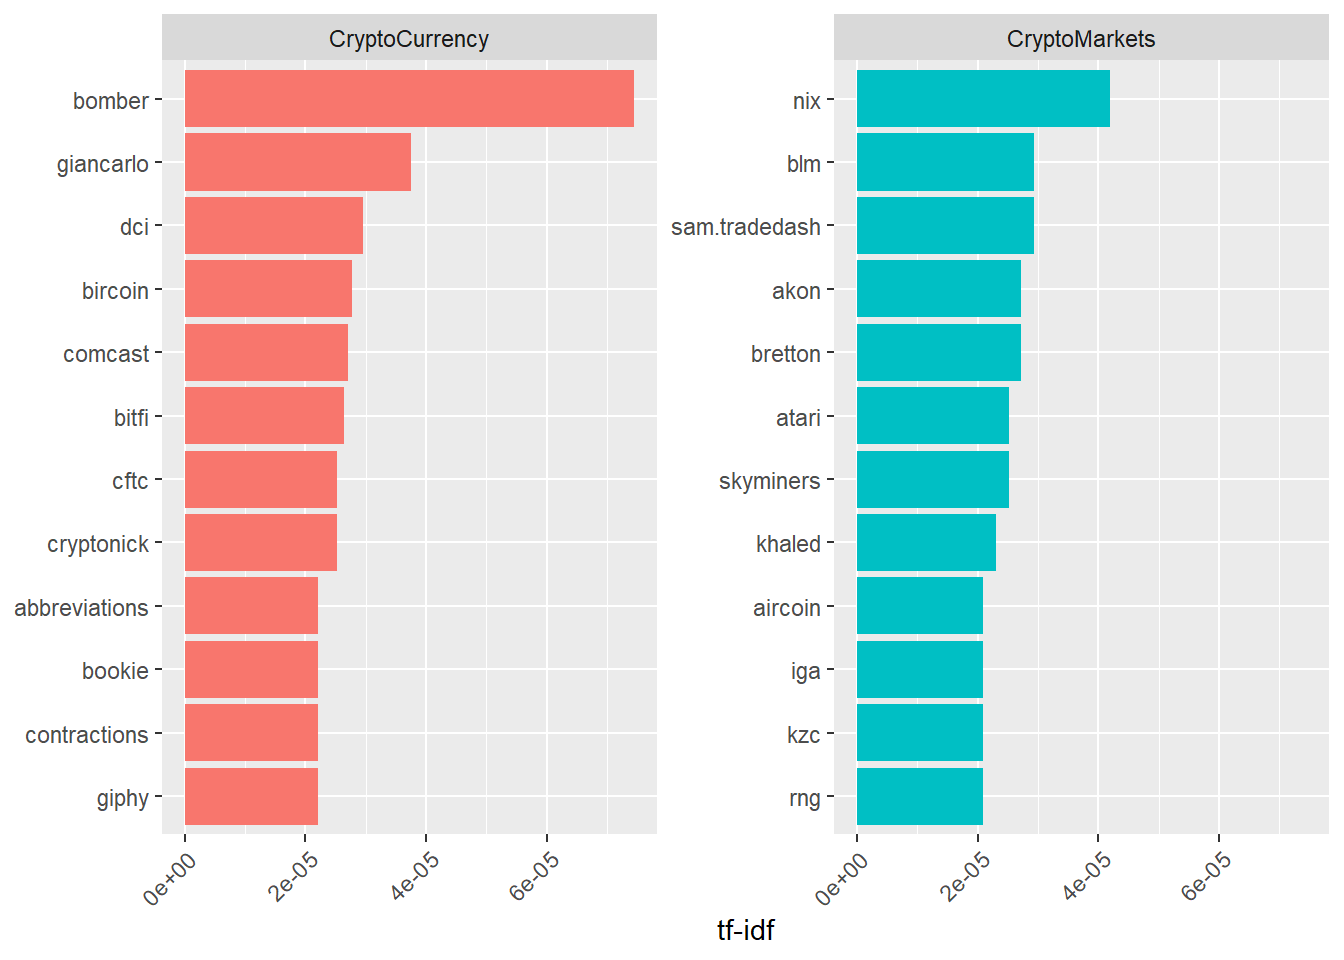
\includegraphics{bookdown-demo_files/figure-latex/all tf_idf-1.pdf}

\begin{Shaded}
\begin{Highlighting}[]
\KeywordTok{ggsave}\NormalTok{(}\StringTok{"tf_idf.pdf"}\NormalTok{, }\DataTypeTok{device =} \StringTok{"pdf"}\NormalTok{, }\DataTypeTok{path =} \StringTok{"CCViz"}\NormalTok{, }\DataTypeTok{height =} \DecValTok{8}\NormalTok{, }\DataTypeTok{width =} \DecValTok{6}\NormalTok{)}
\end{Highlighting}
\end{Shaded}

\hypertarget{posts-over-time}{%
\section{Posts over time}\label{posts-over-time}}

\begin{Shaded}
\begin{Highlighting}[]
\NormalTok{TknsByDate <-}\StringTok{ }\NormalTok{TknsC }\OperatorTok
\StringTok{  }\KeywordTok{separate}\NormalTok{(created, }\KeywordTok{c}\NormalTok{(}\StringTok{"created"}\NormalTok{, }\StringTok{"time"}\NormalTok{), }\StringTok{" "}\NormalTok{) }\OperatorTok
\StringTok{  }\KeywordTok{mutate}\NormalTok{(}\DataTypeTok{created =} \KeywordTok{ymd}\NormalTok{(created)) }\OperatorTok
\StringTok{  }\KeywordTok{mutate_at}\NormalTok{(}\KeywordTok{vars}\NormalTok{(created), }\KeywordTok{funs}\NormalTok{(year, month, day))}
\end{Highlighting}
\end{Shaded}

\begin{Shaded}
\begin{Highlighting}[]
\NormalTok{TknsByMonth <-TknsByDate }\OperatorTok
\StringTok{    }\KeywordTok{filter}\NormalTok{(year }\OperatorTok{>}\StringTok{ }\DecValTok{2015}\NormalTok{) }\OperatorTok
\StringTok{    }\KeywordTok{mutate}\NormalTok{(}\DataTypeTok{Month =} \KeywordTok{make_date}\NormalTok{(year, month))}

\NormalTok{monthCount <-}\StringTok{ }\NormalTok{TknsByMonth }\OperatorTok
\StringTok{    }\KeywordTok{group_by}\NormalTok{(subreddit, month, year) }\OperatorTok\StringTok{ }\CommentTok{#group words by affiliation label}
\StringTok{    }\KeywordTok{count}\NormalTok{(word, }\DataTypeTok{sort =} \OtherTok{TRUE}\NormalTok{) }\OperatorTok\StringTok{ }\CommentTok{#count and create column 'n'}
\StringTok{    }\KeywordTok{top_n}\NormalTok{(}\DecValTok{10}\NormalTok{, n) }\OperatorTok
\StringTok{    }\KeywordTok{ungroup}\NormalTok{()}

\NormalTok{monthCount <-}\StringTok{ }\NormalTok{monthCount }\OperatorTok
\StringTok{    }\KeywordTok{group_by}\NormalTok{(subreddit, month, year) }\OperatorTok
\StringTok{    }\KeywordTok{mutate}\NormalTok{(}\DataTypeTok{prop =}\NormalTok{ n }\OperatorTok{/}\StringTok{ }\KeywordTok{max}\NormalTok{(n))}
    
\KeywordTok{table}\NormalTok{(monthCount}\OperatorTok{$}\NormalTok{subreddit)}
\end{Highlighting}
\end{Shaded}

\begin{verbatim}
## 
## CryptoCurrency  CryptoMarkets 
##            396            435
\end{verbatim}

\begin{Shaded}
\begin{Highlighting}[]
\KeywordTok{ggplot}\NormalTok{(monthCount, }\KeywordTok{aes}\NormalTok{(}
  \DataTypeTok{label =}\NormalTok{ word,}
  \DataTypeTok{size =}\NormalTok{ prop,}
  \DataTypeTok{color =}\NormalTok{ prop}
\NormalTok{)) }\OperatorTok{+}
\StringTok{  }\KeywordTok{geom_text_wordcloud_area}\NormalTok{(}\DataTypeTok{rm_outside =} \OtherTok{TRUE}\NormalTok{) }\OperatorTok{+}
\StringTok{  }\KeywordTok{scale_size_area}\NormalTok{(}\DataTypeTok{max_size =} \DecValTok{20}\NormalTok{) }\OperatorTok{+}
\StringTok{  }\CommentTok{#scale_colour_gradient2(low = "black", mid = "red4", high = "red", space = "Lab", aesthetics = "color") +}
\StringTok{  }\KeywordTok{theme_minimal}\NormalTok{() }\OperatorTok{+}
\StringTok{  }\KeywordTok{facet_grid}\NormalTok{(}\KeywordTok{vars}\NormalTok{(month), }\KeywordTok{vars}\NormalTok{(year))}
\end{Highlighting}
\end{Shaded}

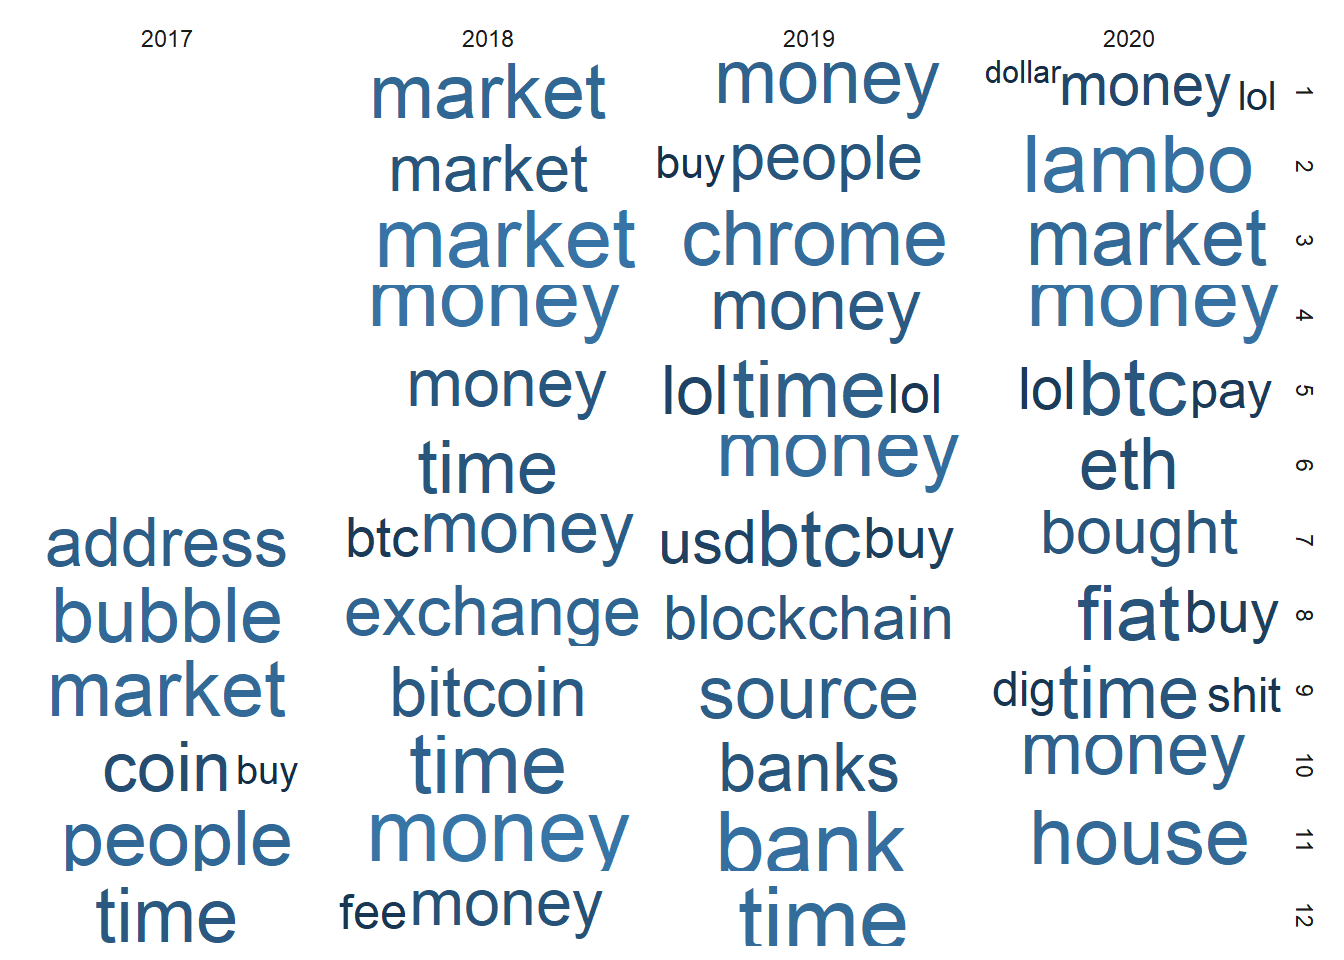
\includegraphics{bookdown-demo_files/figure-latex/unnamed-chunk-20-1.pdf}

\begin{Shaded}
\begin{Highlighting}[]
\KeywordTok{ggsave}\NormalTok{(}
  \StringTok{"CC_timeline.pdf"}\NormalTok{,}
  \DataTypeTok{device =} \StringTok{"pdf"}\NormalTok{,}
  \DataTypeTok{path =} \StringTok{"CCViz"}\NormalTok{,}
  \DataTypeTok{height =} \DecValTok{30}\NormalTok{,}
  \DataTypeTok{width =} \DecValTok{20}
\NormalTok{)}
\end{Highlighting}
\end{Shaded}

\hypertarget{currencies}{%
\section{Currencies}\label{currencies}}

\begin{Shaded}
\begin{Highlighting}[]
\NormalTok{BTC <-}\StringTok{ }\KeywordTok{c}\NormalTok{(}\StringTok{"Bitcoin"}\NormalTok{, }\StringTok{"bitcoin"}\NormalTok{, }\StringTok{"BTC"}\NormalTok{, }\StringTok{"btc"}\NormalTok{)}
\NormalTok{ETH <-}\StringTok{ }\KeywordTok{c}\NormalTok{(}\StringTok{"Ethereum"}\NormalTok{, }\StringTok{"ethereum"}\NormalTok{, }\StringTok{"ETH"}\NormalTok{, }\StringTok{"eth"}\NormalTok{)}
\NormalTok{XRP <-}\StringTok{ }\KeywordTok{c}\NormalTok{(}\StringTok{"Ripple"}\NormalTok{, }\StringTok{"ripple"}\NormalTok{, }\StringTok{"XRP"}\NormalTok{, }\StringTok{"xrp"}\NormalTok{)}
\NormalTok{LTC <-}\StringTok{ }\KeywordTok{c}\NormalTok{(}\StringTok{"Litecoin"}\NormalTok{, }\StringTok{"litecoin"}\NormalTok{, }\StringTok{"LTC"}\NormalTok{, }\StringTok{"ltc"}\NormalTok{)}
\NormalTok{LINK <-}\StringTok{ }\KeywordTok{c}\NormalTok{(}\StringTok{"Chainlink"}\NormalTok{, }\StringTok{"chainlink"}\NormalTok{, }\StringTok{"LINK"}\NormalTok{, }\StringTok{"link"}\NormalTok{)}

\NormalTok{currencies <-}\StringTok{ }\KeywordTok{c}\NormalTok{(BTC, ETH, XRP, LTC, LINK)}

\CommentTok{# For frequency analysis}
\NormalTok{CurTkns <-}\StringTok{ }\NormalTok{TknsByDate }\OperatorTok
\StringTok{  }\KeywordTok{filter}\NormalTok{(word }\OperatorTok\StringTok{ }\NormalTok{currencies)}

\CommentTok{# For sentiment analysis}
\NormalTok{CurComms <-}\StringTok{ }\NormalTok{CommData }\OperatorTok
\StringTok{  }\KeywordTok{filter}\NormalTok{(comm_id }\OperatorTok\StringTok{ }\NormalTok{CurTkns}\OperatorTok{$}\NormalTok{comm_id)}
\end{Highlighting}
\end{Shaded}

\hypertarget{assigning-identifiers}{%
\subsection{Assigning Identifiers}\label{assigning-identifiers}}

\begin{Shaded}
\begin{Highlighting}[]
\NormalTok{CurTkns <-}\StringTok{ }\NormalTok{CurTkns }\OperatorTok
\StringTok{  }\KeywordTok{mutate}\NormalTok{(}\DataTypeTok{Coin =} \KeywordTok{case_when}\NormalTok{(}
\NormalTok{    .}\OperatorTok{$}\NormalTok{word }\OperatorTok\StringTok{ }\NormalTok{BTC }\OperatorTok{~}\StringTok{ "BTC"}\NormalTok{,}
\NormalTok{    .}\OperatorTok{$}\NormalTok{word }\OperatorTok\StringTok{ }\NormalTok{ETH }\OperatorTok{~}\StringTok{ "ETH"}\NormalTok{,}
\NormalTok{    .}\OperatorTok{$}\NormalTok{word }\OperatorTok\StringTok{ }\NormalTok{XRP }\OperatorTok{~}\StringTok{ "XRP"}\NormalTok{,}
\NormalTok{    .}\OperatorTok{$}\NormalTok{word }\OperatorTok\StringTok{ }\NormalTok{LTC }\OperatorTok{~}\StringTok{ "LTC"}\NormalTok{,}
\NormalTok{    .}\OperatorTok{$}\NormalTok{word }\OperatorTok\StringTok{ }\NormalTok{LINK }\OperatorTok{~}\StringTok{ "LINK"}
\NormalTok{  ))}
\end{Highlighting}
\end{Shaded}

\begin{Shaded}
\begin{Highlighting}[]
\NormalTok{curTknsByMonth <-CurTkns }\OperatorTok
\StringTok{    }\KeywordTok{mutate}\NormalTok{(}\DataTypeTok{Month =} \KeywordTok{make_date}\NormalTok{(year, month))}

\NormalTok{curCounts <-}\StringTok{ }\NormalTok{curTknsByMonth }\OperatorTok
\StringTok{    }\KeywordTok{group_by}\NormalTok{(Coin) }\OperatorTok\StringTok{ }\CommentTok{#group words by affiliation label}
\StringTok{    }\KeywordTok{count}\NormalTok{(word, }\DataTypeTok{sort =} \OtherTok{TRUE}\NormalTok{) }\OperatorTok\StringTok{ }\CommentTok{#count and create column 'n'}
\StringTok{    }\KeywordTok{ungroup}\NormalTok{()}

\NormalTok{curCountsbyMonth <-}\StringTok{ }\NormalTok{curTknsByMonth }\OperatorTok
\StringTok{    }\KeywordTok{group_by}\NormalTok{(Coin, Month) }\OperatorTok\StringTok{ }\CommentTok{#group words by affiliation label}
\StringTok{    }\KeywordTok{count}\NormalTok{(word, }\DataTypeTok{sort =} \OtherTok{TRUE}\NormalTok{) }\OperatorTok\StringTok{ }\CommentTok{#count and create column 'n'}
\StringTok{    }\KeywordTok{ungroup}\NormalTok{()}
\end{Highlighting}
\end{Shaded}

\begin{Shaded}
\begin{Highlighting}[]
\KeywordTok{ggplot}\NormalTok{(curCounts) }\OperatorTok{+}
\StringTok{  }\KeywordTok{geom_bar}\NormalTok{(}\KeywordTok{aes}\NormalTok{(}\DataTypeTok{x =}\NormalTok{ Coin, }\DataTypeTok{y =}\NormalTok{ n, }\DataTypeTok{fill =}\NormalTok{ Coin), }\DataTypeTok{stat =} \StringTok{"identity"}\NormalTok{)}
\end{Highlighting}
\end{Shaded}

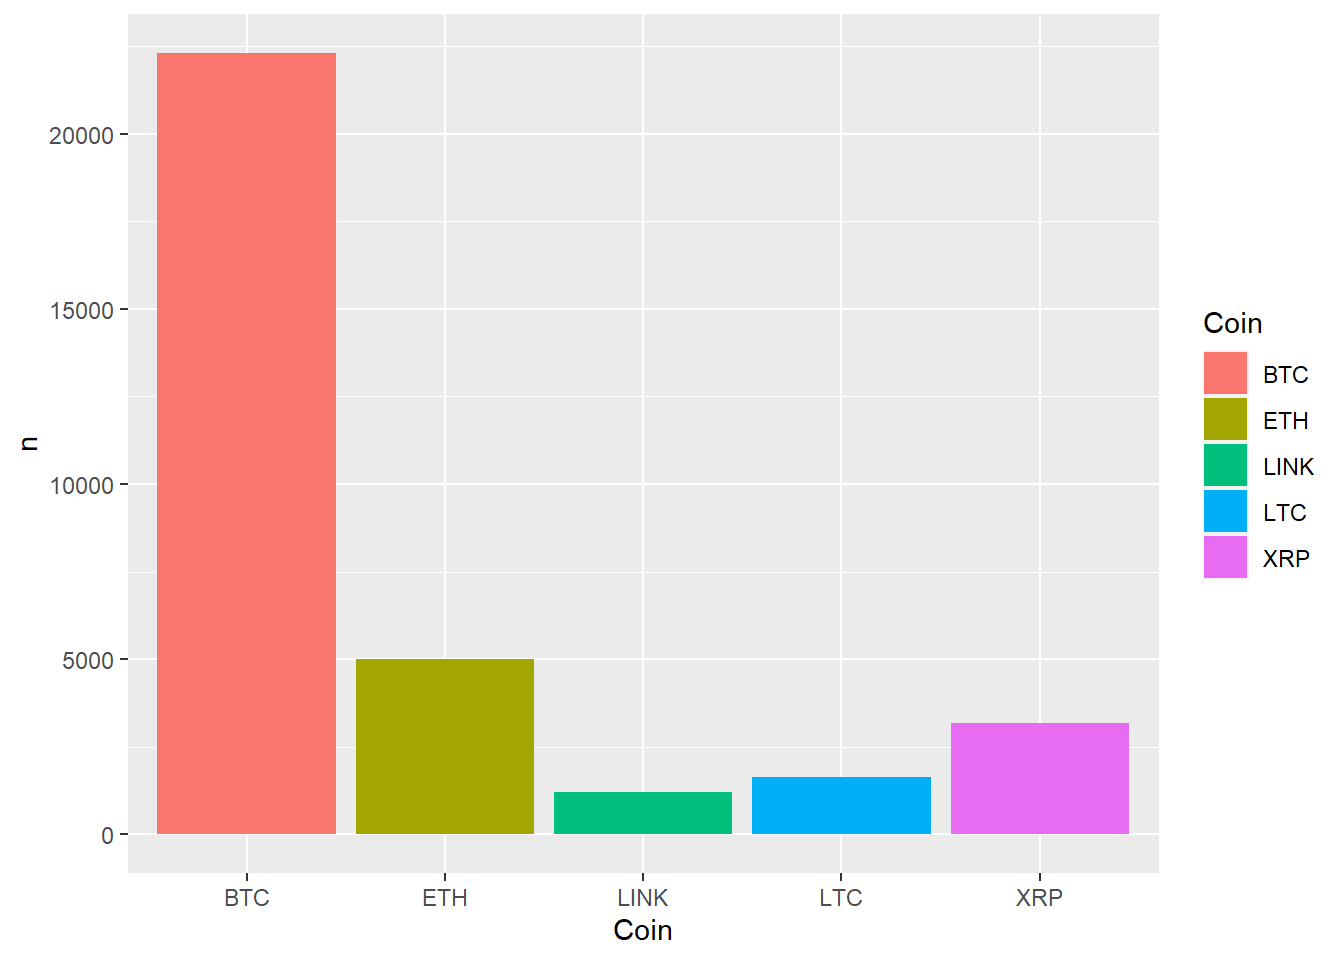
\includegraphics{bookdown-demo_files/figure-latex/unnamed-chunk-24-1.pdf}

\begin{Shaded}
\begin{Highlighting}[]
\KeywordTok{ggplot}\NormalTok{(curCountsbyMonth) }\OperatorTok{+}
\StringTok{  }\KeywordTok{geom_bar}\NormalTok{(}\KeywordTok{aes}\NormalTok{(}\DataTypeTok{x =}\NormalTok{ Coin, }\DataTypeTok{y =}\NormalTok{ n, }\DataTypeTok{fill =}\NormalTok{ Coin), }\DataTypeTok{stat =} \StringTok{"identity"}\NormalTok{) }\OperatorTok{+}
\StringTok{  }\KeywordTok{facet_wrap}\NormalTok{(}\OperatorTok{~}\NormalTok{Month)}
\end{Highlighting}
\end{Shaded}

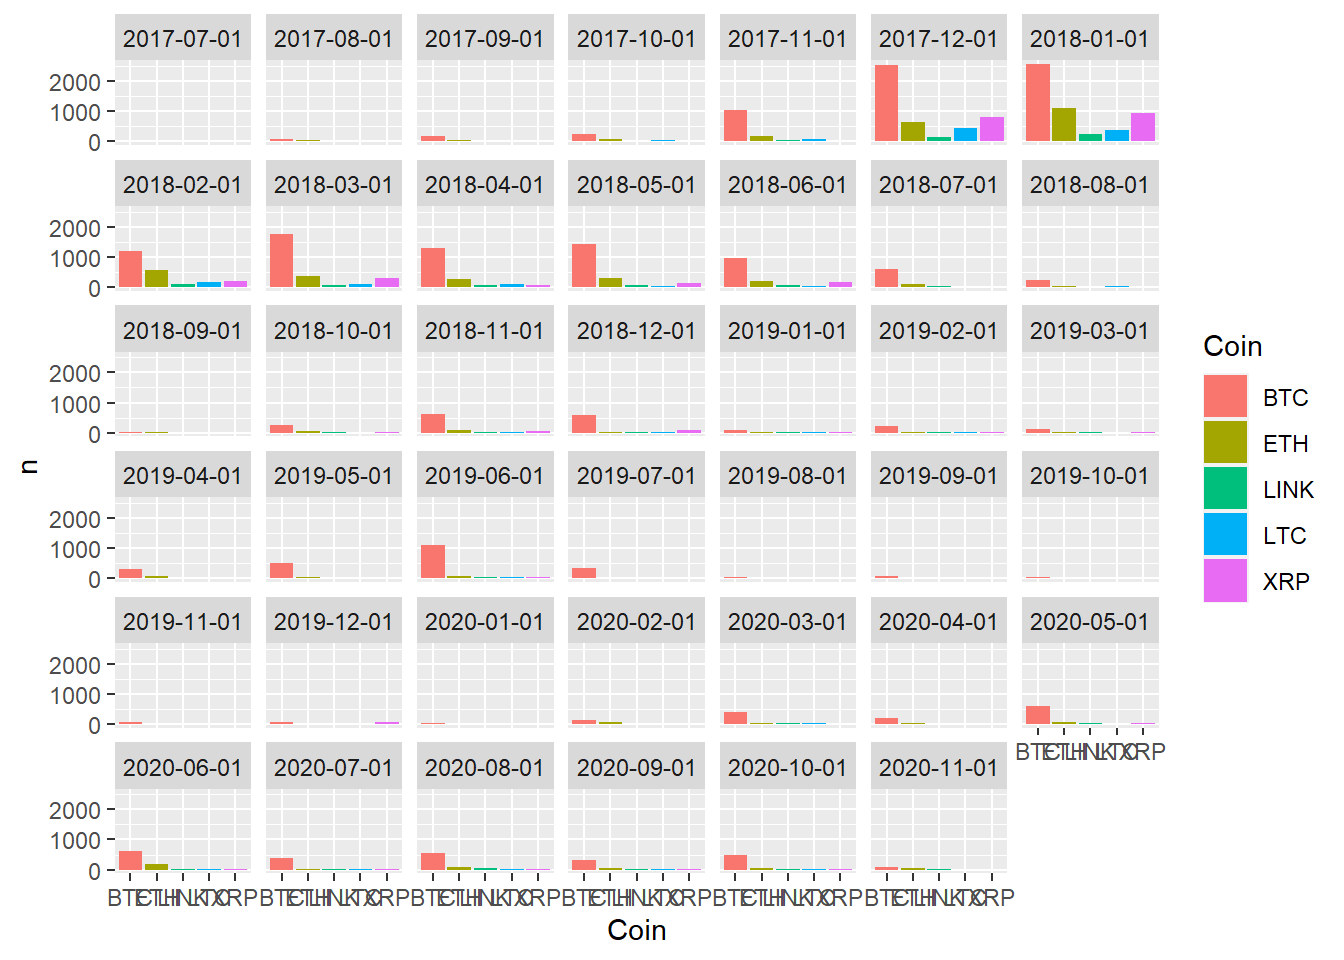
\includegraphics{bookdown-demo_files/figure-latex/unnamed-chunk-25-1.pdf}

  \bibliography{book.bib,packages.bib}

\end{document}
